\documentclass{article}

\usepackage{project-format/project_440_550}
\usepackage[utf8]{inputenc}
\usepackage[T1]{fontenc}
\usepackage[USenglish]{babel}
\usepackage{csquotes}
\usepackage{booktabs}
\usepackage{amsmath}
\usepackage{amsfonts}
\usepackage{microtype}
\usepackage{xcolor}
\usepackage{hyperref}
\usepackage{url}
\usepackage{graphicx}
\usepackage[style=authoryear,maxbibnames=30,natbib]{biblatex}
\addbibresource{refs.bib}
\renewbibmacro{in:}{}
\DeclareDelimFormat{nameyeardelim}{\addspace}
\DeclareNameAlias{sortname}{given-family}
\usepackage[capitalize,noabbrev]{cleveref}

\title{A Per-Pitcher Bake-Off for Next-Pitch Prediction Using 2025 MLB Statcast Data}

\author{%
  Rowan Cake\\
  43367440
}

\begin{document}
\maketitle

\begin{abstract}
This project follows the \emph{application bake-off} track from the course proposal specification: one application, next-pitch prediction in Major League Baseball, is evaluated with a range of machine learning methods under a common experimental pipeline. Using a cleaned 2025 Statcast dataset of 325{,}611 pitches from 30 pitchers, the study trains pitcher-specific models to predict the next pitch type from pre-pitch context and recent within-at-bat history. The final bake-off compares multinomial logistic regression, k-nearest neighbors, hidden Markov model style transition baselines, linear and Gaussian discriminant analysis, LSTM, 1D CNN, and XGBoost. XGBoost performs best with mean per-pitcher test accuracy of 41.76\%, followed by the Markov baseline at 40.34\%, while deep sequence models do not outperform the stronger non-neural baselines. Although the absolute accuracy is lower than originally hoped, the bake-off shows that the task is substantially harder under a realistic chronological split on modern Statcast data, and suggests that feature design and distribution shift matter more than model complexity alone.
\end{abstract}

\section{Introduction}
Predicting the next pitch in baseball is an appealing machine learning problem because it combines structured game context, short-range sequential dependence, and genuine strategic uncertainty. The task is also practically meaningful: even a modest improvement in anticipating pitch type could be useful for coaching, player analysis, or decision support. Public pitch-by-pitch tracking systems such as Statcast make this problem accessible at scale by recording game state, player handedness, runner configuration, and pitch metadata for every MLB game \citep{statcast}.

For this course project, the chosen track was the \emph{application bake-off} described in the project proposal document: select a specific application and compare a range of techniques, with the contribution being evidence about which methods work better for that application and why. The application here is \emph{per-pitcher next-pitch prediction} using the 2025 MLB regular season. Rather than introducing a new model class, the main contribution is a careful empirical comparison of several standard methods from the course and adjacent literature under one consistent pipeline.

The central question is straightforward: given only information available \emph{before} the current pitch is thrown, how well can the pitcher's next pitch type be predicted? Modern models, especially sequence models, might be expected to improve substantially over simple baselines. In practice, that did not happen. The best model improved only modestly over a naive most-common-pitch baseline, and deep models did not dominate. This negative result is still useful: it clarifies the difficulty of the problem under realistic evaluation and helps identify where the main bottlenecks likely lie.

\section{Related Work}
Prior baseball pitch prediction work has often reported stronger accuracies than those obtained here, but usually under different data, label spaces, or evaluation settings. \citet{hamilton2014applying} studied pitch prediction using PITCHf/x data from the 2008--2009 seasons and several classical classifiers. Their setting was primarily binary fastball versus non-fastball prediction, which is substantially easier than modern multi-class prediction, and they also used pitcher/count-specific feature selection. This line of work established that pre-pitch context contains signal, but it does not directly answer how difficult fine-grained multi-class prediction is on newer data.

\citet{sidle2018multiclass} moved closer to the present task by evaluating multi-class prediction for individual pitchers using linear discriminant analysis, support vector machines, and classification trees on 2013--2015 data. They reported mean out-of-sample accuracy of 66.62\% for their best method, which is far above the results in this project. However, their data filtering, pitch taxonomy, and historical setting differ meaningfully from the present study, and their paper highlights how much performance depends on pitcher-specific distributions and the choice of evaluation baseline.

\citet{lee2022ensemble} proposed an ensemble of deep neural networks to jointly predict pitch type and pitch location. Their emphasis was on richer output structure rather than purely pitcher-specific modeling, and the paper argues that predicting both type and location is more practically useful than type alone. That work is relevant because it motivates trying stronger nonlinear models, but it also studies a different formulation and a different notion of generalization.

Relative to this literature, my project is less about beating published numbers and more about conducting a controlled bake-off on a new 2025 Statcast-derived dataset under a chronological split. In that sense, the most relevant comparison is not paper-to-paper accuracy, but how several common models behave when faced with the same modern data pipeline.

\section{Data and Experimental Setup}
\subsection{Dataset Construction}
The input to all experiments was a cleaned dataset stored in \texttt{processed/phase1\_cleaned\_all\_pitchers.csv}, derived from 2025 regular-season Statcast data. The final dataset contained 325{,}611 pitches from 30 starting pitchers. Each row corresponded to one pitch and included only features that were available before the current pitch was thrown.

The final target for the main bake-off was \texttt{target\_pitch\_type}. I also built infrastructure for location prediction, but the later stages of the project focused on pitch type because that was the more stable and informative target.

\subsection{Features}
The feature set was intentionally restricted to pre-pitch contextual information. Numeric features included game year, inning, outs, balls, strikes, at-bat number, pitch number, base-runner indicators, score differential, time through the order, prior plate appearances in the game, rest-day variables, and batter/pitcher age. Categorical features included handedness, inning half, home and away teams, and defensive alignment fields.

For sequence-aware models, I also used up to the previous five pitches from the same at-bat. Each historical step contained the prior pitch's pre-pitch context together with one-hot encodings of the prior pitch type and prior location bucket. The current pitch's own pitch type and location were never included in the input.

\subsection{Evaluation Protocol}
All models were trained separately for each pitcher. The split was chronological at the game level: the earliest 80\% of games for a pitcher were used for training and the latest 20\% for testing. This choice is stricter than a random split and better reflects deployment, but it also introduces seasonal drift in pitch usage.

For each pitcher-task pair, target classes with fewer than 20 rows were removed before training. If fewer than two classes remained, the task was skipped. Two pitchers were skipped by most models because the chronological test split contained a pitch class that never appeared in that pitcher's training period. Metrics were averaged across trained pitchers only. To contextualize the results, I also computed a naive baseline that always predicts the most common pitch type from the training split for a given pitcher; its mean test accuracy was 37.95\%.

\section{Methods}
The bake-off compared eight pitcher-specific baselines:
\begin{enumerate}
\item \textbf{Multinomial logistic regression}: a one-layer PyTorch softmax classifier on standardized and one-hot encoded context features.
\item \textbf{k-nearest neighbors}: a nonparametric baseline using flattened recent-history features.
\item \textbf{Hidden Markov model style baseline}: a supervised transition model using recent pitch-history statistics and smoothed conditional counts.
\item \textbf{Linear discriminant analysis (LDA)}: a shared-covariance generative classifier on flattened context and history features.
\item \textbf{Gaussian discriminant analysis (GDA)}: implemented as regularized class-specific covariance modeling with PCA compression before quadratic discriminant analysis.
\item \textbf{LSTM}: a sequence model over the previous five pitches, concatenated with current static context.
\item \textbf{1D CNN}: temporal convolutions over the same within-at-bat history, combined with a static context branch.
\item \textbf{XGBoost}: a tree-based classifier on flattened recent-history and current-context features.
\end{enumerate}

Some methods proposed in the original project idea, such as SVMs and ensemble stacking across models, were not completed. Rather than present partial or unverified results, I restricted the report to methods that were fully implemented, trained, and evaluated in a consistent way.

\section{Results}
\cref{fig:leaderboard,tab:results} summarize the main bake-off outcome. XGBoost was the best model by mean per-pitcher accuracy, with the HMM-style baseline second. LDA was competitive and slightly outperformed both sequence neural networks on accuracy. The LSTM and 1D CNN achieved nearly identical results, but neither improved on XGBoost or the simpler transition baseline.

\begin{figure}[t]
  \centering
  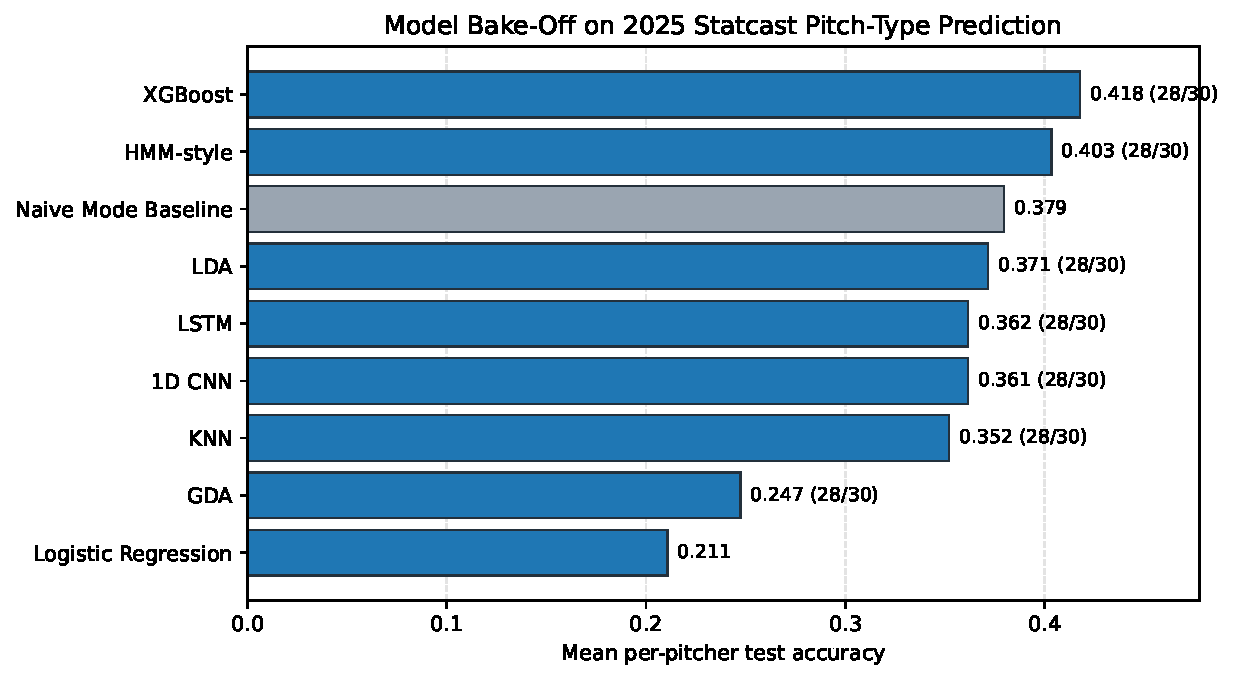
\includegraphics[width=\linewidth]{figures/model_leaderboard.pdf}
  \caption{Mean per-pitcher pitch-type accuracy for all evaluated models. The naive baseline always predicts the most common training-set pitch type for a pitcher.}
  \label{fig:leaderboard}
\end{figure}

\begin{table}[t]
\caption{Pitch-type prediction results on the chronological per-pitcher test split. Precision and recall are macro-averaged across pitch classes.}
\label{tab:results}
\centering
\small
\begin{tabular}{lrrrr}
\toprule
Method & Trained & Accuracy & Precision & Recall \\
\midrule
Naive mode baseline & 30 & 0.3795 & -- & -- \\
Logistic regression & 30 & 0.2107 & 0.2262 & \textbf{0.3159} \\
KNN & 28 & 0.3521 & 0.1951 & 0.1844 \\
HMM-style baseline & 28 & 0.4034 & \textbf{0.2818} & 0.2241 \\
LDA & 28 & 0.3714 & 0.2490 & 0.2410 \\
GDA & 28 & 0.2474 & 0.1958 & 0.2144 \\
LSTM & 28 & 0.3616 & 0.2220 & 0.2139 \\
1D CNN & 28 & 0.3613 & 0.2419 & 0.2356 \\
XGBoost & 28 & \textbf{0.4176} & 0.2676 & 0.2394 \\
\bottomrule
\end{tabular}
\end{table}

Several observations stand out. First, the problem is genuinely difficult under this split: the best model improved over the naive baseline by only about 3.8 percentage points. Second, more expressive neural models did not automatically help. The LSTM and CNN both trained successfully, but their mean accuracy stayed near 36\%, below both XGBoost and the Markov baseline. Third, the gap between LDA and GDA suggests that estimating separate covariance structure for each class is unstable in this feature space even with regularization, likely due to sparsity and class imbalance.

The per-pitcher results also varied substantially. \Cref{fig:xgb-vs-mode} shows that XGBoost generally improved on the naive pitcher-specific baseline, but often only modestly. Under XGBoost, the strongest cases included Kevin Gausman (57.9\%), Framber Valdez (54.4\%), and Corbin Burnes (51.5\%), while pitchers such as Merrill Kelly (31.3\%) and Miles Mikolas (32.2\%) were much harder. This spread reinforces the intuition that predictability is highly pitcher dependent.

\begin{figure}[t]
  \centering
  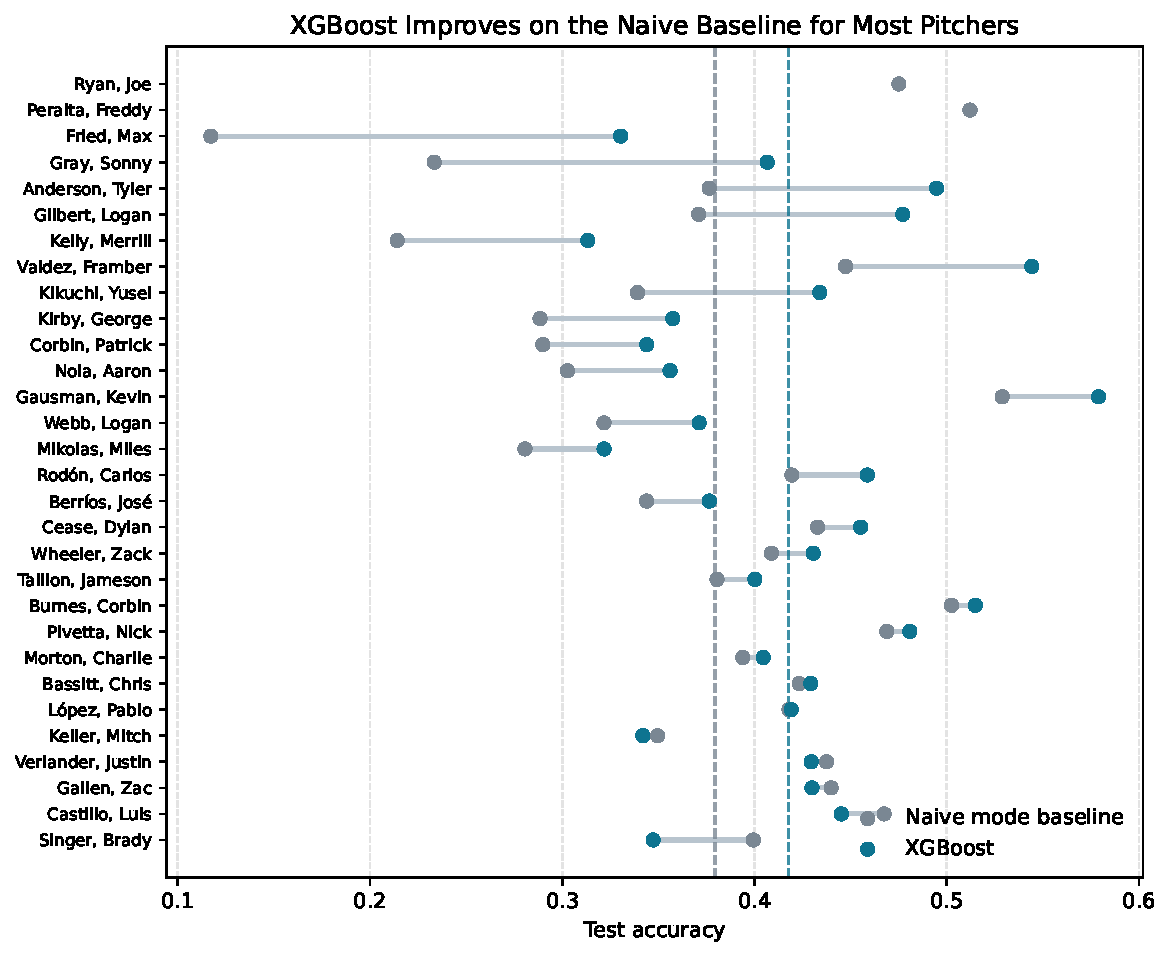
\includegraphics[width=0.96\linewidth]{figures/xgboost_vs_mode.pdf}
  \caption{Pitcher-by-pitcher comparison between the naive mode baseline and the best-performing model, XGBoost. The gains are usually positive, but often small.}
  \label{fig:xgb-vs-mode}
\end{figure}

\section{Discussion}
The main conclusion is that the application bake-off produced a clear ranking of methods, but not the level of predictive accuracy initially expected. On this 2025 dataset, XGBoost was the strongest method, with HMM-style transition modeling surprisingly competitive. Deep sequence models did not justify their additional computational cost: the full 1D CNN run took roughly ten hours and still failed to beat XGBoost or the Markov baseline.

There are three likely reasons for the relatively modest performance. First, pitch choice is intrinsically stochastic and strategic; even with count, handedness, runners, and recent history, pitchers intentionally avoid becoming too predictable. Second, the chronological split induces real distribution shift. Pitch usage can change over a season because of health, coaching adjustments, repertoire changes, or opponent-specific planning. Third, the current features omit some likely high-value signals, especially batter identity, richer matchup history, and broader game-level sequence summaries beyond the last five pitches of the current at-bat.

This project still makes a useful contribution in the sense intended by the bake-off track. It shows that, on a modern pitcher-specific Statcast dataset with realistic temporal evaluation, stronger models do \emph{not} necessarily dominate, and that carefully engineered non-neural baselines remain hard to beat. It also provides a reproducible pipeline and a set of negative results that help narrow down what is worth trying next.

\section{Future Work}
With more time, the first priority would be better feature design rather than deeper architectures. The most promising directions are adding batter identity and rolling matchup statistics, predicting coarser pitch families before exact pitch type, and giving tree-based models richer recent-history aggregates. A second direction would be to revisit the task definition itself: predicting pitch location jointly with pitch type, or predicting pitch family first and subtype second, may align better with the actual information structure available to hitters.

The proposal originally aimed for very high accuracy and a broader model suite. The final outcome is more modest, but also more informative. The evidence from this project suggests that the next gains will likely come from better representation of baseball context rather than simply using a larger neural network.

\printbibliography

\end{document}
